\documentclass[a4paper,12pt]{article}
\usepackage[utf8]{inputenc}
\usepackage[margin=3cm]{geometry}
\usepackage{amsmath}
\usepackage{amssymb}
\usepackage{amsthm}
\usepackage{fancyhdr}
\usepackage{seminar}
\usepackage{graphicx}
\usepackage{subfigure}
\usepackage{float}
\usepackage{hyperref}
\pagestyle{fancy}


%You can add theorem-like environments (e.g. remark, definition, ...) if you want
\newtheorem{theorem}{Theorem}

\title{Seminar Report of KinectFusion: Real-Time\\Dense Surface Mapping and Tracking} % Replace with your title
\author{Wenliang Peng} % Replace with your name
\institute{Faculty of Informatics - Technische Universit\"{a}t M\"{u}nchen} % Replace with the department you belong to

\makeatletter
\let\runauthor\@author
\let\runtitle\@title
\makeatother
\lhead{\runauthor}
\rhead{\runtitle}


\begin{document}

\maketitle

\begin{abstract}
	The paper "KinectFusion: Real-Time Dense Surface Mapping and Tracking" was published by Microsoft Research and was published in 2011. 
	The method proposed in this paper is a pioneering work based on a low-cost RGB-D camera for real-time reconstruction tracking and reconstruction algorithms suitable for different lighting conditions, creating an important framework for 3D dense reconstruction. This paper shows that this method can accurately obtain tracking and mapping results in real-time in room-sized scenes using only commodity sensors and GPU hardware, which surpassed the solutions proposed using passive computer vision at that time.
\end{abstract}

\section{Introduction}

The introduction is expected to give a short background information about the paper's topic.
It should also provide some context for the presented work as follows:
choose 1--2 papers from the related work section, that are very close to the paper you presented.
Explain in detail how your presented paper is different to those, and what is better about it.
Do not (!) repeat all related papers listed in the paper.

 

\section{Method description}
In this method, a dense reconstruction algorithm using depth maps is created to accurately reconstruct the 3D model in real-time. 
the algorithm pipeline is shown in Figure \ref{figure1}, 
including four parts, namely measurement, pose estimation, reconstruction update, and surface prediction.
\begin{figure}[h] %figure环境,h默认参数是可以浮动,不是固定在当前位置。如果要不浮动,你就可以使用大写float宏包的H参数,固定图片在当前位置,禁止浮动。
    \centering %使图片居中显示
    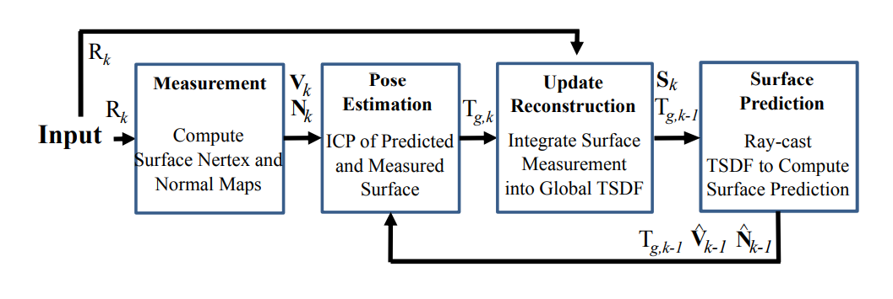
\includegraphics[scale=0.6]{figure1.png} %中括号中的参数是设置图片充满文档的大小,你也可以使用小数来缩小图片的尺寸。
    \caption{Overall system workflow.} %caption是用来给图片加上图题的
    \label{figure1} %这是添加标签,方便在文章中引用图片。
\end{figure}%figure环境

\subsection{Preliminaries}


\subsection{Surface measurement}
\subsection{Pose estimation}
\subsection{Surface reconstruction update}
\subsection{Surface prediction}

\section{Experiments and results}

Try to find a mix between qualitative and quantitative results.
Choose the most meaningful results and describe under what settings they were obtained.
Highlight things that are particularly interesting.
Result figures and tables can be copied from the original papers.

\section{Discussion / Conclusion}

These two points can go together in one section.
Here, you should discuss the results, in particular compared to the related work you mentioned in the introduction.
Also, feel free to write your personal opinion about drawbacks and/or possible extensions of the presented paper.

\section*{Additional remarks about the report}

\begin{itemize}
	\item You are not expected to implement the methods described in the paper you have been assigned.
	\item Please use citations when appropriate. If you use any figures or tables, please make sure you cite the original paper. Add your citations in bibtex format into the file \texttt{egbib.bib}. An example is \cite{newcombe11ismar}.
	\item Please keep all your formulas numbered. You can use the equation environment for this:
	Please use the equation environment to get automatic equation numbering:
		\begin{equation}
		SE(3)$x_{k-1}$ = \left\{
		\begin{pmatrix}
		R & \mathbf{t} \\ \mathbf{0} & 1
		\end{pmatrix}
		:
		R^\top R = R R^\top = I_3, \mathbf{t}\in\mathbb{R}^3
		\right\}
		\end{equation}
	\item The report should be no longer than 4 pages (without citations).
	\item Please do not change the layout (page margins, font size, etc.).
\end{itemize}

\bibliographystyle{plain}
\bibliography{report}



\end{document}